%%%%%%%%%%%%%%%%%%%%%%%%%%%%%%%%%%%%%%%%%%%%%%%%%%%%%%%%%%%%%%%%%%%%%%%%%%%%%%%%%%%%%%%%%%%%%%%%%%%
%%%%%%%%%%%%%%%%%%%%%%%%%%%%%%%%%%%%%%%%%%%%%%%%%%%%%%%%%%%%%%%%%%%%%%%%%%%%%%%%%%%%%%%%%%%%%%%%%%%
%%%%%%%%%%%%%%%%%%%%%%%%%%%%%%%%%%%%%%%%%%%%%%%%%%%%%%%%%%%%%%%%%%%%%%%%%%%%%%%%%%%%%%%%%%%%%%%%%%%
%%%%%%%%%%%%%%%%%%%%%%%%%%%%%%%%%%%%%%%%%%%%%%%%%%%%%%%%%%%%%%%%%%%%%%%%%%%%%%%%%%%%%%%%%%%%%%%%%%%

\chapter{Variables aleatorias}

%%%%%%%%%%%%%%%%%%%%%%%%%%%%%%%%%%%%%%%%%%%%%%%%%%%%%%%%%%%%%%%%%%%%%%%%%%%%%%%%%%%%%%%%%%%%%%%%%%%
%%%%%%%%%%%%%%%%%%%%%%%%%%%%%%%%%%%%%%%%%%%%%%%%%%%%%%%%%%%%%%%%%%%%%%%%%%%%%%%%%%%%%%%%%%%%%%%%%%%

\section{Medidas}

Un primer motivo para esta sección es enfatizar que, formalmente, una variable aleatoria se concibe 
como un espacio de medida y no como un recuento de eventos. 
Paralelamente, introducir la terminología adecuada permitirá entender los teoremas que dan base
a los análisis realizados.

\begin{definicion}[$\boldsymbol{\sigma}$-álgebra]
Sea $U$ un conjunto y $\mathcal{U}$ una colección de subconjuntos de $U$. Se dice que $\mathcal{U}$
es una $\sigma$-álgebra si comple que
\begin{itemize}
\item $U \in \mathcal{U}$
\item $A \in \mathcal{U}$ implica que $A^{C} \in \mathcal{U}$
\item Si $\{ A_n \}_{n\in \mathbb{N}}$ son conjuntos tales que $A_i \in \mathcal{U}$, entonces
$\displaystyle \cup_{n\in \mathbb{N}} A_n \in \mathcal{U}$
\end{itemize}
Donde $A^{C}$ es el complemento $\{ u \in U | u \notin A \} $
\end{definicion}

Por simplicidad, en este trabajo sólo se usarán medidas para conjuntos de números reales derivadas 
de la $\sigma$-álgebra de Borel, que es definida como la $\sigma$-álgebra más pequeña que contiene a 
los intervalos abiertos abiertos\footnote{Si una $\sigma$-álgebra contiene a todos los
intervalos abiertos, entonces debe contener a todos los elementos de la $\sigma$-álgebra de Borel}.

\begin{definicion}[Medida]
Sea $U$ un conjunto y $\mathcal{U}$ una $\sigma$-álgebra definida en $U$. Se dice que una función
$\mu : \mathcal{U} \rightarrow \R \cup {\infty}$ es una medida si cumple que
\begin{itemize}
\item $\mu(\emptyset) = 0$
\item $\mu(A) \geq 0$ para cualquier $A \in \mathcal{U}$
\item Si $\{ A_n \}_{n\in \mathbb{N}}$ son conjuntos disjuntos a pares y tales que 
$A_i \in \mathcal{U}$, entonces 
$\displaystyle \mu\left( \cup_{n\in \mathbb{N}} A_n \right) = \sum_{n\in \mathbb{N}} \mu(A_n)$
\end{itemize}
Donde $\emptyset$ es el conjunto vacío %y $\R^{*} = \R \cup \{-\infty,\infty \}$
\end{definicion}

\begin{definicion}[Medida de probabilidad en $\boldsymbol{\R}$]
Sea $\mathcal{B}$ la sigma álgebra de Borel definida para $\R$, se dice que una función
$P : \mathcal{B} \rightarrow [0.1]$ es una \textbf{medida de probabilidad} si cumple que
\begin{itemize}
\item $P(\emptyset) = 0$
\item $0 \leq P(A) \leq 1$ para cualquier $A \in \mathcal{B}$
\item Si $A, B \in \mathcal{B}$ y $A\cap B = \emptyset$, entonces $P(A \cup B) = P(A) + P(B)$ 
\item $P(\R) = 1$
\end{itemize}
\label{variable_aleatoria}
\end{definicion}

%Cabe mencionar que cuando se usa una variable aleatoria para modelar un fenómeno, existe un paso
%intermedio en que los eventos relevantes se asocian con números reales

Otra forma de entender una variables aleatoria es a partir de su función de probabilidad
acumulada (FPA), ya que hay una correspondencia unívoca entre cada variable aleatoria y su FPA.

\begin{definicion}[Función de Probabilidad Acumulada]
Sea 
\begin{equation*}
F_X (x) = P\left( (-\infty,x] \right)
\end{equation*}
\end{definicion}

Habitualmente, como se hace el presente texto, se usa el símbolo $X$ para denotar a una variable 
aleatoria cuya FDA es $F_X$; bajo esta idea, para cualquier conjunto $I \subseteq \R$ se denota
$P(X \in I) = P(I)$



\begin{teorema}[Descomposici\'on de Lebesgue]
Sea $f:I\rightarrow \R$ una funci\'on de variaci\'on acotada, con $I$ un intervalo. Entonces pueden 
hallarse funciones $f_j, f_c, f_a :I\rightarrow \R$ tales que
\begin{itemize}
\item $f = f_j+ f_c+ f_a$
\item $f_j = \sum_{y \leq x} f(x-0) + f(x+0)$
\item $f_a$ es absolutamente continua\footnote{Para que una funci\'on sea absolutamente continua,
basta que sea de variaci\'on acotada y que mapee conjuntos de medida cero en conjuntos de medida
cero} en $I$
\item $f_c$ es una funci\'on singular\footnote{Una funci\'on es singular si es continua, de 
variaci\'on acotada y no-constante, y se cumple que tiene derivada cero casi en todas partes} en 
$I$
\end{itemize}
Estas funciones son \'unicas excepto por constantes, y en conjunto son llamados la 
\textit{descomposici\'on de Lebesgue} de $f$
\label{Lebesgue_decomp}
\end{teorema}

%%%%%%%%%%%%%%%%%%%%%%%%%%%%%%%%%%%%%%%%%%%%%%%%%%%%%%%%%%%%%%%%%%%%%%%%%%%%%%%%%%%%%%%%%%%%%%%%%%%

\section{Procesos estocásticos}

Una forma natural de pensar en la definici\'on \ref{cont_est} es que, si $\abso{t-t_0}$ es muy 
peque\~no, entonces $X(t)$ y $X(t_0)$ difieren muy poco entre s\'i (como variables aleatorias).
Es destacable que si un proceso es estoc\'asticamente continuo en un intervalo, sus realizaciones 
solamente se pueden garantizar continuas casi en todas partes \footnote{Una propiedad se cumple 
\textbf{casi en todas partes} si se cumple en un conjunto cuyo complemento tiene medida cero} en 
ese intervalo.

Como ejemplos, un proceso ruido blanco (definici\'on \ref{r_blanco}) no es estoc\'asticamente 
continuo, mientras que un proceso de Wiener (definici\'on \ref{r_wiener}) s\'i lo es.

\begin{definicion}[Proceso ruido blanco]
Se dice de un proceso estoc\'astico $\{ R(t) \}$ que cumple, para cualesquiera tiempos admisibles
$t$ y $s$, las siguientes propiedades:
\begin{itemize}
\item $\E{R(t)}=0$
\item $\Cov{R(t),R(s)}=0 \Leftrightarrow t=s$ 
\end{itemize}
\label{r_blanco}
\end{definicion}

\begin{definicion}[Proceso de Wiener]
Se dice de un proceso estoc\'astico $\{ W(t) \}$ que cumple, para cualesquiera tiempos admisibles
$t$ y $s$ (con $s>t$) las siguientes propiedades:
\begin{itemize}
\item $W(0) = 0$ ($W(0)$ es constante)
\item $W(s)-W(t)$ es independiente de $W(u)$, para todo $u<t$ admisible
\item $W(s)-W(t) \sim N(0,\abso{t-s})$  (los incrementos tienen distribuci\'on normal)
\end{itemize}
\label{r_wiener}
\end{definicion}


\section{Periodograma}

Una observaci\'on interesante sobre estos teoremas es el caso $\tau = 0$
\begin{equation*}
\rho(0) = \int_{-A}^{+A} dF(\omega) = F(A) - F(-A)
\end{equation*}
donde $A$ vale $\infty$ o $\pi$ seg\'un sea el caso discreto o continuo. Si $R$ es la funci\'on de
autocovarianza del proceso, entonces la ecuaci\'on anterior se traduce en que
\begin{equation*}
R(0) = \sigma^{2} \left( F(A) - F(-A) \right) = \sigma^{2} F(A)
\end{equation*}
donde $\sigma^{2}$ es la varianza del proceso. 
Esta observaci\'on adquiere importancia porque la FDE integrada ($H$), por definici\'on, satisface 
el papel de $F$ salvo por la condici\'on $F(\infty)=1$; si se puede garantizar que 
$H(\infty)<\infty$ entonces puede ser normalizada para satisfacer tal condici\'on y, m\'as a\'un,
si tal fuera el caso entonces $H(\infty)=\sigma^{2}$. Una consecuencia muy fuerte de este 
comentario es que, como se ha establecido previamente que s\'olo se considerar\'an procesos con
segundos momentos finitos, entonces la FDE de los procesos considerados siempre es acotada.


Se puede demostrar que $\aste{R}$ tiene las siguientes propiedades:
\begin{itemize}
\item $\E{\aste{R}(\tau)} = \left(1 - \frac{\abso{\tau}}{N} \right) R(\omega)$
\item $\Var{\aste{R}(\tau)} \approx \frac{1}{N} 
\sum_{r=-\infty}^{\infty} \left( R^{2}(r) + R(r-\tau)R(r+\tau) \right)$
\item $\Cov{\aste{\rho}(\tau),\aste{\rho}(\tau+\nu)} \approx \frac{1}{N} 
\sum_{r=-\infty}^{\infty} \left( \rho(r)\rho(r+\nu) + \rho(r-\tau)\rho(r+\tau+\nu) \right)$
\end{itemize}
Las aproximaciones para la varianza y covarianza se vuelven exactas si el proceso sigue una 
distribuci\'on normal en todos los tiempos.

%%%%%%%%%%%%%%%%%%%%%%%%%%%%%%%%%%%%%%%%%%%%%%%%%%%%%%%%%%%%%%%%%%%%%%%%%%%%%%%%%%%%%%%%%%%%%%%%%%%

\subsection{Representación espectral}

\begin{teorema}
Sea $\{X(t)\}$ un proceso estoc\'astico a tiempo continuo d\'ebilmente estacionario de media 0 y 
estoc\'asticamente continuo en el sentido de media cuadr\'atica. Entonces, existe un proceso 
ortogonal $\{Z(\omega)\}$ tal que, para todo tiempo $\omega$ admisible, se puede 
escribir\footnote{La integral se encuentra definida en el sentido de media cuadr\'atica.}
\begin{equation*}
X(t) = \intR e^{i t \omega} dZ(\omega)
\end{equation*}
Donde el proceso $\{Z(t)\}$ tiene las siguientes propiedades para todo $\omega$
\begin{itemize}
\item $\E{dZ(\omega)} = 0$
\item $\E{\abso{dZ(\omega)}^{2}} = dH(\omega)$
\item $\Cov{dZ(\omega),dZ(\lambda)} = 0 \Leftrightarrow \omega \neq \lambda$
\end{itemize}
Donde $dH(\omega)$ la FDE integrada de $\{X(t)\}$
%\label{rep_espectral}
\end{teorema}

En virtud del teorema de Wold, se puede tener una variante del teorema \ref{rep_espectral}
para procesos a tiempo discreto, raz\'on por la cual  
tal representaci\'on es referida como \textbf{representaci\'on de Wold-Cram\'er}.

%%%%%%%%%%%%%%%%%%%%%%%%%%%%%%%%%%%%%%%%%%%%%%%%%%%%%%%%%%%%%%%%%%%%%%%%%%%%%%%%%%%%%%%%%%%%%%%%%%%
%%%%%%%%%%%%%%%%%%%%%%%%%%%%%%%%%%%%%%%%%%%%%%%%%%%%%%%%%%%%%%%%%%%%%%%%%%%%%%%%%%%%%%%%%%%%%%%%%%%
%%%%%%%%%%%%%%%%%%%%%%%%%%%%%%%%%%%%%%%%%%%%%%%%%%%%%%%%%%%%%%%%%%%%%%%%%%%%%%%%%%%%%%%%%%%%%%%%%%%

\begin{SidewaysTable}
\centering
\bordes{1.5}
\begin{tabular}{c}
\textbf{Ventanas de retrasos tipo escalamiento (1)}
\vspace{1em}
\end{tabular}

{
\begin{tabular}{lll}
\toprule
& $k(u)$ para $\abso{u} \leq 1$ & \\
\midrule
Bartlett &
$\displaystyle 
1 
$
& 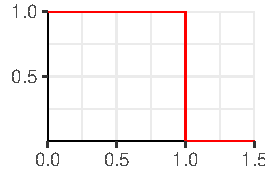
\includegraphics[scale=.66]{./img_ventanas/ventana_bartlett.pdf}
\\
\rowcolor{gris}
Fejer &
$\displaystyle 
1-\abso{u}
$
& 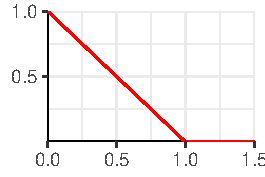
\includegraphics[scale=.66]{./img_ventanas/ventana_fejer.pdf}
\\
Daniell &
$\displaystyle 
\frac{\SEN{\pi u}}{\pi u}
$
& 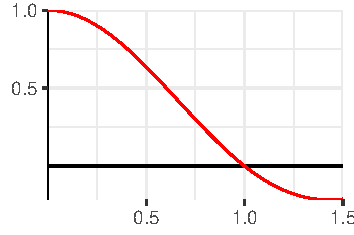
\includegraphics[scale=.66]{./img_ventanas/ventana_daniell.pdf}
\\
\rowcolor{gris}
Parzen (1) &
$\displaystyle 
1-u^{2}
$
& 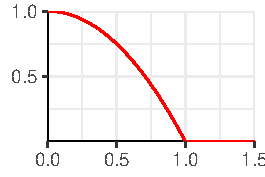
\includegraphics[scale=.66]{./img_ventanas/ventana_parzen1.pdf}
\\
Parzen (2) &
$\displaystyle 
\frac{1}{1+\abso{u}}
$
& 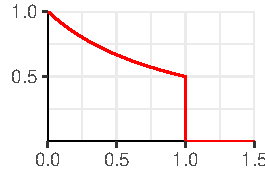
\includegraphics[scale=.66]{./img_ventanas/ventana_parzen2.pdf}
\\
\rowcolor{gris}
Parzen (3) &
$\displaystyle 
\frac{1}{1+u^{2}}
$
& 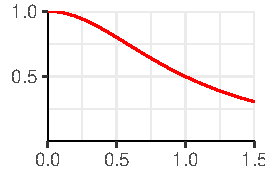
\includegraphics[scale=.66]{./img_ventanas/ventana_parzen3.pdf}
\\
Parzen (4) &
$\displaystyle 
\begin{cases}
1-6 u^{2} + 6 \abso{u}^{3} &, \text{ si} \abso{u}\leq \nicefrac{1}{2}\\
2\left( 1-\abso{u} \right)^{3} &, \text{ otro caso}
\end{cases}
$
& 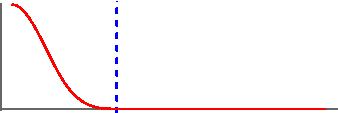
\includegraphics[scale=.66]{./img_ventanas/ventana_parzen4.pdf}
\\
\rowcolor{gris}
Tukey &
$\displaystyle 
1 -2a +2a \COS{\pi u}
$
& 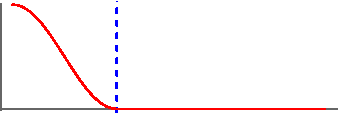
\includegraphics[scale=.66]{./img_ventanas/ventana_tukey.pdf}
\\
\bottomrulec
\end{tabular}
}
\caption{Ejemplos de algunas ventanas que suavizan el periodograma}
\label{ventanas}
\end{SidewaysTable}

%%%%%%%%%%%%%%%%%%%%%%%%%%%%%%%%%%%%%%%%%%%%%%%%%%%%%%%%%%%%%%%%%%%%%%%%%%%%%%%%%%%%%%%%%%%%%%%%%%%

\begin{SidewaysTable}
\centering
\bordes{1.5}
\begin{tabular}{c}
\textbf{Ventanas de retraso tipo escalamiento (2)}
\vspace{1em}
\end{tabular}

{
\begin{tabular}{lll}
\toprule
& $k(u)$ para $\abso{u} \leq 1$  & \\
\midrule
Neave &
$\displaystyle 
\begin{cases}
1 &, \abso{u}\leq a \\
\frac{1}{1-a}\left[ 1-u +\frac{b-a}{\pi}\SEN{\frac{b-u}{b-a}\pi} \right] &, a \leq \abso{u}\leq a \\
\frac{1}{1-a}\left[ 1-u -\frac{1-b}{\pi}\SEN{\frac{u-b}{1-b}\pi} \right] &, b \leq \abso{u} \\
\end{cases}
$
& 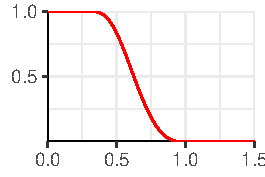
\includegraphics[scale=.66]{./img_ventanas/ventana_neave.pdf}
\\
\rowcolor{gris}
Cuadrática &
$\displaystyle 
\frac{25}{12(\pi u)^{2}} 
\left[ \frac{\SEN{\nicefrac{6 \pi u}{5}}}{\nicefrac{6\pi u}{5}} - \COS{\nicefrac{6 \pi u}{5}} \right]
$
& 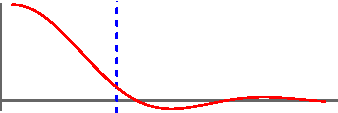
\includegraphics[scale=.66]{./img_ventanas/ventana_cuadratica.pdf}
\\
Bartlett-Priestley &
$\displaystyle 
\frac{3}{(\pi u)^{2}} \left[ \frac{\SEN{\pi u}}{\pi u} - \COS{\pi u} \right]
$
& 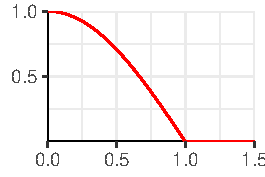
\includegraphics[scale=.66]{./img_ventanas/ventana_cosenoidal.pdf}
\\
\rowcolor{gris}
Papoulis &
$\displaystyle 
(1-u)\COS{\pi u} + \frac{\SEN{\pi u }}{\pi u }
$
& 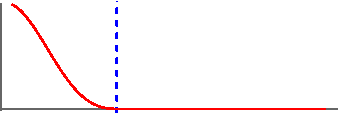
\includegraphics[scale=.66]{./img_ventanas/ventana_papoulis.pdf}
\\
Cosenoidal &
$\displaystyle 
\COS{\pi u}
$
\\
\rowcolor{gris}
Trapezoidal &
$\displaystyle 
\begin{cases}
1 &, \abso{u}\leq a \\
\frac{u-1}{a-1} &, a \leq \abso{u}\leq a 
\end{cases}
$
& 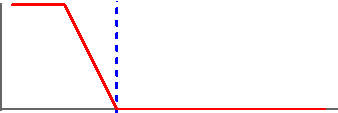
\includegraphics[scale=.66]{./img_ventanas/ventana_trapezoidal.pdf}
\\
Normal &
$\displaystyle 
\exp \left( - \nicefrac{u^{2}}{2 \sigma^{2}}  \right)
$
%& 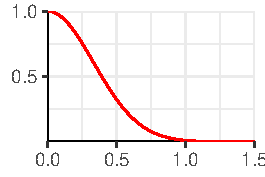
\includegraphics[scale=.66]{./img_ventanas/ventana_normal.pdf}
& 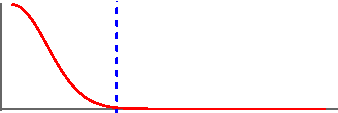
\includegraphics[scale=.66]{./img_ventanas/ventana_.pdf}
\\
\bottomrule
\end{tabular}
}
\caption{Ejemplos de algunas ventanas que suavizan el periodograma}
\end{SidewaysTable}

%%%%%%%%%%%%%%%%%%%%%%%%%%%%%%%%%%%%%%%%%%%%%%%%%%%%%%%%%%%%%%%%%%%%%%%%%%%%%%%%%%%%%%%%%%%%%%%%%%%
%%%%%%%%%%%%%%%%%%%%%%%%%%%%%%%%%%%%%%%%%%%%%%%%%%%%%%%%%%%%%%%%%%%%%%%%%%%%%%%%%%%%%%%%%%%%%%%%%%%
%%%%%%%%%%%%%%%%%%%%%%%%%%%%%%%%%%%%%%%%%%%%%%%%%%%%%%%%%%%%%%%%%%%%%%%%%%%%%%%%%%%%%%%%%%%%%%%%%%%

\begin{SidewaysTable}
\centering
\bordes{1.5}
\begin{tabular}{c}
\textbf{Ventanas espectrales tipo escalamiento (1)}
\vspace{1em}
\end{tabular}

{
\begin{tabular}{ll}
\toprule
& $K(\theta)$ para $\abso{\theta} \leq 1$ \\
\midrule
Bartlett &
$\displaystyle 
\frac{1}{\pi} \frac{\SEN{\theta}}{\theta}
$
\\
\rowcolor{gris}
Fejer &
$\displaystyle 
\frac{1}{2\pi} \left[ \frac{\SEN{\nicefrac{\theta}{2}}}{\nicefrac{\theta}{2}} \right]^{2}
$
\\
Daniell &
$
\displaystyle 
\nicefrac{1}{2\pi} \text{, si } \abso{\theta}\leq \pi
$
\\
\rowcolor{gris}
Parzen (1) &
$\displaystyle 
d
$
\\
Parzen (2) &
$\displaystyle 
d
$
\\
\rowcolor{gris}
Parzen (3) &
$\displaystyle 
d
$
\\
Parzen (4) &
$\displaystyle 
\frac{3}{8 \pi} \left[ \frac{\SEN{\nicefrac{\theta}{4}}}{\nicefrac{\theta}{4}} \right]
$
\\
\rowcolor{gris}
Tukey &
$\displaystyle 
d
$
\\
\bottomrulec
\end{tabular}
}
\caption{Ejemplos de algunas ventanas que suavizan el periodograma}
\end{SidewaysTable}

%%%%%%%%%%%%%%%%%%%%%%%%%%%%%%%%%%%%%%%%%%%%%%%%%%%%%%%%%%%%%%%%%%%%%%%%%%%%%%%%%%%%%%%%%%%%%%%%%%%

\begin{SidewaysTable}
\centering
\bordes{1.5}
\begin{tabular}{c}
\textbf{Ventanas de retraso tipo escalamiento (2)}
\vspace{1em}
\end{tabular}

{
\begin{tabular}{ll}
\toprule
& $K(\theta)$ para $\abso{\theta} \leq 1$ \\
\midrule
Neave &
$
d
$
\\
\rowcolor{gris}
Cuadrática &
$\displaystyle 
d
$
\\
Bartlett-Priestley &
$\displaystyle 
\frac{3}{4 \pi} \left[ 1 - \left( \nicefrac{\theta}{\pi} \right) \right]
\text{, si } \abso{\theta}\leq \pi
$
\\
\rowcolor{gris}
Papoulis &
$\displaystyle 
d
$
\\
Coseno &
$\displaystyle 
d
$
\\
\rowcolor{gris}
Trapezoidal &
$\displaystyle 
d
$
\\
Normal &
$\displaystyle 
d
$
\\
\bottomrule
\end{tabular}
}
\caption{Ejemplos de algunas ventanas que suavizan el periodograma}
%\label{ventanas}
\end{SidewaysTable}

%%%%%%%%%%%%%%%%%%%%%%%%%%%%%%%%%%%%%%%%%%%%%%%%%%%%%%%%%%%%%%%%%%%%%%%%%%%%%%%%%%%%%%%%%%%%%%%%%%%
%%%%%%%%%%%%%%%%%%%%%%%%%%%%%%%%%%%%%%%%%%%%%%%%%%%%%%%%%%%%%%%%%%%%%%%%%%%%%%%%%%%%%%%%%%%%%%%%%%%
%%%%%%%%%%%%%%%%%%%%%%%%%%%%%%%%%%%%%%%%%%%%%%%%%%%%%%%%%%%%%%%%%%%%%%%%%%%%%%%%%%%%%%%%%%%%%%%%%%%
%%%%%%%%%%%%%%%%%%%%%%%%%%%%%%%%%%%%%%%%%%%%%%%%%%%%%%%%%%%%%%%%%%%%%%%%%%%%%%%%%%%%%%%%%%%%%%%%%%%